% Metódy inžinierskej práce

\documentclass[10pt,twoside,english,a4paper]{article}

\usepackage[english]{babel}
%\usepackage[T1]{fontenc}
\usepackage[IL2]{fontenc} % lepšia sadzba písmena Ľ než v T1
\usepackage[utf8]{inputenc}
\usepackage{graphicx}
\usepackage{url} % príkaz \url na formátovanie URL
\usepackage{hyperref} % odkazy v texte budú aktívne (pri niektorých triedach dokumentov spôsobuje posun textu)
\usepackage{tabularx}

\usepackage{cite}
%\usepackage{times}


\pagestyle{headings}

\title{Modelling UX and UI for human-machine interaction design for mobile applications\thanks{Predbežná verzia článku v predmete Metódy inžinierskej práce, ak. rok 2021/22, vedenie: Fedor Lehocki}} % meno a priezvisko vyučujúceho na cvičeniach

\author{Vasko Mykhailo\\[2pt]
	{\small Slovenská technická univerzita v Bratislave}\\
	{\small Fakulta informatiky a informačných technológií}\\
	{\small \texttt{xvaskom@stuba.sk}}
	}

\date{\small 14 December 2021} % upravte


\begin{document}

\maketitle

%\begin{abstract}
%\ldots 1)	I chose this theme because User Interface and Experience is very important in usage of an app, and good UX can achieve very good interaction effect, and hope it will help to get understanding how to build responsive and comfortable UX and UI for mobile apps.
%
%2)	Good UI and UX are in demand now as never before. “As the relationship between humans and technology continues to evolve, it’s more important than ever for businesses to emphasize UX design in mobile app development initiatives. Truly understanding a product’s user, researching to solve user pain-points, learning about latent behaviors and needs is the only way to ensure exceptional product performance”. ~\cite{WinNT}
%
%3)	The problem is apps that have amazing functional and great possibilities in commercialization but because of bad UI or UX don’t have or lose users. \cite{Examples}
%
%4)	Simplest solution is to hire UI and UX designers to a project, that will do research and design for product, but I’m here to educate developers to understand steps to make good User Design and Interface and how it is made.
%
%5)	 A lot of apps have amazing design, because they have done a lot of research, analysis and design on top of experimenting with it.
%
%6)	This article is about all stages of modelling and creating up-to-date design of an app from scratch and ways to make it better. 
%
%
%\end{abstract}



\section{Introduction}

Comfort in usage of your favorite app, or ease of use in the app you just downloaded- these are examples of good combination of UX and UI. But sometimes apps that have amazing functional and great possibilities in commercialization struggle because of bad UI or UX, don’t have or lose users or don't get enough attention.
Division of Computer and Mechatronics Engineering, Sahmyook University, Korea, conducted research of understanding of UI and UX. . It was found that excellent was 19.35\%, average was 42.53\% and insufficient was 38.12\%. Therefore, only 20\% of the students understood UI/UX well...\cite{UnderstandingUI}
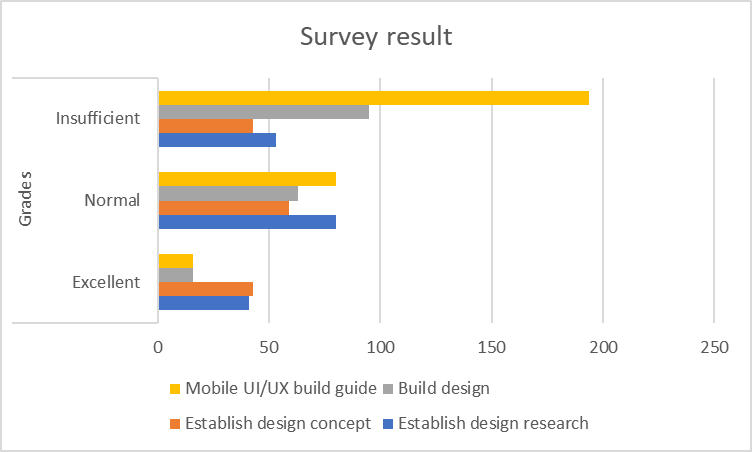
\includegraphics[width=1\textwidth]{diagram.png}

 Today I will tell about User Experience and User Interface design in mobile apps and why it’s so important in using app and viewing content\cite{Examples}. 
 The purpose of this text is to help understand the importance of UI and UX design, show the main differences between them and how it’s usually created, answer a lot UX and UI questions for newbies and explain some features.


\section{Difference between UX and UI} \label{UX/UI}
\subsection{Difference}

UX stands for User Experience. It describes certain experience user gets interacting with interface of an app. It responds for ease of use and simplicity: if user can find some function and go back quickly and easily, UX is done well.

UI is the User Interface – appearance of the interface and its characteristics: styling, color scheme, physical characteristics (where elements should be) and other sections like suitability of color range and how elements work together, will for user be convenient to hit that button. 

The common misconception is that these two fields are common and interchangeable. UX is a core of an app, it focuses on success of use in general. The UX designer plans how you interact with the interface and what steps you need to take to get something done. And the UI designer comes up with how each of these steps will look like. In the workflow, the UX is done first, and then the UI. As you can see from the examples above, UX and UI are so closely related that sometimes the line between concepts is blurred\cite{WhatIsDesign}.

\subsection{History}
The profession of UX/UI designer has existed for a long time, it just wasn't called like that before. More precisely, before it was not called at all, but was part of other professions.

Here’s an example: when Wilhelm Schickard invented arithmometer, he was already a UX/UI designer, due to the fact he was the one who designed which tumblers and in what sequence a person should turn in order to get the end result of the calculations. He additionally found out in what logical order they might be located. He found out how most of these pens might look. He created an interface for interacting with the machine\cite{WhatIsDesign}.



\section{User Interface} \label{UI}
\subsection{Principles} 
User interface design is an essential a part of the display screen products. According to psychology, we can divide interface design into two levels: visual and emotional. There are three principles of User interface design: the user interface to under control, Reduce the burden of user memory, maintain the consistency of the interface. Feeling level between man and machine refers to the visual, auditory aspect and touch. Emotional level refers to communicate between man and machine because of a harmonious relationship. User interface design flow into the structure design, interaction design, and visual design of three components in the work\cite{5681254}.

\begin{itemize}
\item Structure design
\begin{enumerate}

\item Interface with the color and style is unified interface system: general color should close software and system interface. Certainly reasonable combination is system interface design including icons, button style in different operating conditions and the visual effects.
\item Unique interface framework: interface architecture, securities trading and map manipulation interface characteristics goes in pace with with industry standards.
	\end{enumerate}
\item Interactive design

Interaction design aims to make the products so that users can simply use, simplify user operation flow. Therefore, the human factor should be the core of the design.

\item Visual design

Pleasing visible layout used to achieve the purpose of the user. Coherent interface should be the size for aesthetic point of view, feel comfortable and coordination, can be effective to attract the user's attention within. At the same time colors of interface closely connected with color theory and color harmony…
\end{itemize}

\subsection{Design process}
Consists of few steps: 
\begin{itemize}
%\item         Context and user recognition
%\item         Navigational and systemic interface design
%\item        Distributional design of interface
\item Confirm target customer
\item Research habits of target's interaction
\item Develop structure design
\item Develop interactive design
\item Develop visual design
\item Test usability of the prototype
\item Products prototype design - follow the usability: software should be understandable, achievable and controllable by user. \cite{5681254}
\end{itemize}

\subsection{Trends}
UI design is a dynamic field that brings us new trends every year. These are some trends in UI that are likely to dominate next few years:
\begin{itemize}
\item Minimalistic UI
\item Neumorphism
\item Asymmetry
\item Negative space
\item Imperfect elements
\item 3D elements and parallax
\item Rich color and sensuous typography
\item Long scrolling and parallax technique websites 
\cite{UItrends}
\cite{UnderstandingUI}
\end{itemize}

\section{User Experience} \label{UX}
\subsection{Methods}
The most used method of developing UX nowadays is waterfall method, other ones are Agile and HCD(Human-centered design).

\cite{WaterfallUX}
\subsection{Stages of creating}	
\begin{center}
\begin{tabular}{ |c|c| } 
 \hline
 Waterfall & Human-centered design \\ 
\hline\hline
 1.Requirements & 1.Creating UX vision \\ 
\hline
 2.Design & 2.Creating high-level concept \\ 
 \hline
3.Implementation& 3.Designing and developing the interaction and visual style\\ 
 \hline 
4.Validation & 4.Evaluating the design against requirements\\ 
 \hline
5.Maintenance&  \\ 
 \hline
\end{tabular}
\end{center}
\cite{AllUX}
\begin{enumerate}
\item Creating UX Vision : goal is to define UX vision as a high level understanding of the user value the app will deliver to the end user, it will help in determining the essence of the app for the user. When the purpose of an app is already known, it’s not always necessary.
\item Creating a High-Level Concept : it can be a drawing or a prototype, visual presentation that makes the vision more concrete and helps to connect it. 
\item Designing and Developing Interaction and Visual Style : the moment when starts UI developing, when conceptual user flow refining to an implementable design.
\item Evaluating UX of the Outcome : scope the project to simple and focused functions customers really need, dropping unneeded features that will slow down the project and take costs.\cite{Kuusinen2014}
\end{enumerate}

\subsection{Trends}

\section{Discussion}
Although mobile app development tend to be much faster than development of a desktop applications, it seems easier to have more flexible processes and roles, but it’s not always right. Most of the times you can get better result having two different people being responsible for UX and UI, because UX specialist is the one who needs to know style guides for every platform, and UI designer is expert at things like aesthetics and platform design therefore can make design much more appealing.
\subsection{Future of UI and UX}
UX, as part of service industry, will only gain popularity and spread to new markets as health infrastructure, along with the fact that TVs, tablets and phones will evolving and the demand for them does not decreases. Artificial intelligence and machine learning will help designers generating thousands of variants of logos or layouts, but the main role will be left behind man, because affective user research and user testing, for instance, are complex and require emotional intelligence and, importantly, an ability to understand needs and behaviors.

Also Voice User Interfaces become more popular every year:  Apple has Siri, Google has Google Assistant, Microsoft has Cortana, and Amazon has Alexa. It’s likely that users will find voice interfaces valuable in situations where visual attention or touch interaction are occupied.
\cite{FutureDesign}
\subsection{Qualities of the UX designer of tomorrow}
\begin{itemize}
\item Adaptable

The past decade of change shows us that design must constantly adapt as a discipline, in order to meet new client, customer, and user needs, but some core principles will stay for a long time. Skills like user research, user journey design, wireframes, prototypes, high-fidelity visual design, user testing, and even coding won't be superfluous.
\item Detail-oriented, but capable of seeing the big picture

Employers will look for detail-oriented UX designers who can deliver improvements at the micro level to upgrade existing design but also to appraise wider design, tech, and market trends, and scan the horizon for possible changes.\cite{DesignerTomorrow}
\end{itemize}

\section{Conclusion}
The first step to solving any task is to define it. Understanding the
differences between UI and UX will help you more competently approach design projects, distribute work and correctly lead the process of creating a design. There are few principles and concepts that you should keep in mind designing an app, that I wrote in this article, and they will help you create the very good design that everyone strives for.	\cite{Kuusinen2014} Also user interface and experience gradually become more widespread and known and although very promising direction, it is now one of the most demanded design professions in the digital industry. How long it will be in demand depends on the development of this industry. And, apparently, it is only gaining momentum.

%\acknowledgement{Ak niekomu chcete poďakovať\ldots}

%\DeclareUnicodeCharacter{Ukrainian} \cite{beregovyi2019difference}





%% týmto sa generuje zoznam literatúry z obsahu súboru literatura.bib podľa toho, na čo sa v článku odkazujete
\bibliography{literatura}
\bibliographystyle{plain} % prípadne alpha, abbrv alebo hociktorý iný
\end{document}
